\chapter{Lecture 19: Antiderivatives of more complicated functions II}
In the previous lecture we introduced integration by parts, as the antiderivative analogue of the product rule. Now we introduce integration by substitution. \\

\noindent Integration by substitution is the antiderivative analogue of the chain rule. We can use it to integrate functions which involve compositions of two functions. However, we will soon see that the types of functions that we can integrate by substitution need to satisfy some extra conditions (they do not only involve compositions).

\section{Integration by substitution} \label{integration by substitution 1}
We now derive the integration by substitution rule from the chain rule. For the product rule, our notation involved using $f(x)$ and $f'(x)$, where $f(x)$ was an antiderivative of $f'(x)$. To make the integration by substitution rule neater we will use $F(x)$ and $f(x)$, where $F(x)$ is an antiderivative of $f(x)$; both ways mean the same thing, it is just a matter of preference in notation. \\

\noindent The chain rule is
\[
\frac{d}{dx}\brac{F(g(x))} = f(g(x))g'(x)
\]
Integrating both sides gives
\[
\int \frac{d}{dx}\brac{F(g(x))} \; dx = \int f(g(x))g'(x) \; dx
\]
The antiderivative cancels the derivative on the left hand side, giving the integration by substitution rule (we also swapped the sides of the equality):

  	\bigskip
	
	\hfil\fbox{
	\begin{minipage}{0.35\columnwidth}{
	
	\vskip 0.02cm
	\begin{center}
	$\displaystyle{\int f(g(x))g'(x) \; dx = F(g(x))}$
	\end{center}
	}
	\end{minipage}}
	\bigskip

\noindent Sometimes you will see this written differently, as follows: If we let $g(x) = u$, then $g'(x) = \frac{du}{dx}$, and $F(g(x)) = F(u)$. So we write

  	\bigskip
	
	\hfil\fbox{
	\begin{minipage}{0.35\columnwidth}{
	
	\vskip 0.02cm
	\begin{center}
	$\displaystyle{\int f(u)\frac{du}{dx} \; dx = F(u)}$
	\end{center}
	}
	\end{minipage}}
	\bigskip

\noindent There is another very common way to write it, which may help with your understanding and memory, so we have to include it here. It is important to realise that $F(u)$ really means ``the antiderivate of $f(u)$,'' i.e., $F(u) = \int f(u) \; du$. Hence you will often see the integration by substitution rule written:

  	\bigskip
	
	\hfil\fbox{
	\begin{minipage}{0.35\columnwidth}{
	
	\vskip 0.02cm
	\begin{center}
	$\displaystyle{\int f(u)\frac{du}{dx} \; dx = \int f(u) \; du}$
	\end{center}
	}
	\end{minipage}}
	\bigskip

\noindent To help remember this rule, people imagine that they are ``cancelling the $dx$'' from the right hand side, so they pretend that $\displaystyle{\frac{du}{dx}dx = du}.$ \\

\noindent Just to throw in one more way to write it, a personal favourite is

  	\bigskip
	
	\hfil\fbox{
	\begin{minipage}{0.4\columnwidth}{
	
	\vskip 0.02cm
	\begin{center}
	$\displaystyle{\int f(g(x))g'(x) \; dx = \int f(u) \; du}$, where $u = g(x).$
	\end{center}
	}
	\end{minipage}}
	\bigskip

\noindent At first it is troubling having so many ways to write the same thing, then it eventually becomes useful to have some freedom of expression. The important thing is that we understand exactly what the rule is saying. \\

\noindent Usually, we apply this rule by trying to match the left hand side of the rule to the function that we are integrating. So, we need to pick $g(x)$ and $f(x)$ in such a way that the function we are integrating has the form $f(g(x))g'(x)$; or, if you like the other notation better: $f(u)\frac{du}{dx}.$ \\

\noindent As you can see, this form is not simply a ``composition of two functions;'' it is also the product of that composition with the derivative of the inner function, $g(x)$. \\

\noindent For example, the function $h(x) = x\e^{-\frac{1}{2}x^2}$ has the required form: Where $f(x) = \e^{-x}$ and $g(x) = \frac{1}{2}x^2$. So, $f(g(x)) = \e^{-\frac{1}{2}x^2}$ and $g'(x) = \frac{2}{2}x = x$, giving
\[
f(g(x))g'(x) = x\e^{-\frac{1}{2}x^2} = h(x)
\]
This means that
\begin{align*}
\int x\e^{-\frac{1}{2}x^2} \; dx & = \int f(g(x))g'(x) \; dx \\
	& =  \int f(u) \; du   \tag{substitution rule, where $u = g(x)$}\\
	& = \int \e^{-u} \; du \tag{since $f(x) = \e^{-x}$} \\
	& = -\e^{-u} \\
	& = -\e^{-\frac{1}{2}x^2}. \tag{since $u = g(x) = \frac{1}{2}x^2$}
\end{align*}
The function that we just integrated may have looked like a good candidate for integration by parts. However, using integration by parts on this function will lead to problems (try it). A good rule of thumb is to always decide if you can apply integration by substitution first, then use integration by parts otherwise.

\subsection{The simplest type of substitution}
We gave a rule in section \ref{simplest chain} for the simplest application of the chain rule, we now give a rule for the simplest application of substitution. \\

\noindent Just as was the case with the chain rule, the simplest type of substitution is when
\[
h(x) = f(ax+b), \qquad \text{for any real constants $a,b.$}
\] 
We can let $f(ax+b) = f(g(x))$, where $g(x)$ has the form of a straight line, i.e., $g(x) = ax+b$. So,
\[
g'(x) = \frac{d}{dx}\brac{ax+b} = a.
\]
To match the left hand side of the substitution rule, the function we are integrating must have the form $g'(x)f(g(x))$, which in this case would look like
\[
g'(x)f(g(x)) = af(ax+b). \tag{since $g'(x) = a$}
\]
But $h(x) = f(ax+b)$, not $af(ax+b)$; there is no constant, $a$, out front yet. However, multiplying by $\frac{a}{a} = 1$ will fix this, without changing the value of the expression (we are technically just multiplying by 1). Doing this, then using the linearity of integration
\[
\int f(ax+b) \; dx = \int\frac{a}{a} f(ax+b) \; dx = \frac{1}{a} \int af(ax+b) \; dx.
\]
We have
\begin{align*}
\int f(ax+b) \; dx & = \frac{1}{a} \int af(ax+b) \; dx \\
	& = \frac{1}{a} \int g'(x)f(g(x)) \; dx \tag{since $g(x) = ax+b$ and $g'(x) = a$} \\
	& = \frac{1}{a} F(u) \qquad (\bigstar) \tag{letting $u = g(x)$, integration by substitution} \\
	& = \frac{1}{a} \int f(u) \; du. \tag{since $F$ is an antiderivative of $f$}
\end{align*}
Where $u = ax+b$. \\

\noindent For example. Suppose we wish to antidifferentiate $h(x) = (3x+12)^8$. Then $u = 3x+12$, $f(u) = u^8$, and $a = 3$. So $(\bigstar)$ tells us that
\begin{align*}
\int (3x+12)^8 \; dx & = \frac{1}{3} \int f(u) \; du \\
	& = \frac{1}{3} \int u^8 \; du \tag{since $f(u) = u^8$} \\
	& = \frac{1}{3} \frac{1}{9}u^9 \tag{integration formula} \\
	& = \frac{1}{27} (3x+12)^9. \tag{since $u = 3x+12$}
\end{align*}
In practice, you can skip many of the explanatory steps and just ``write down'' the answer once you get used to simple substitution.

\subsection{Simple substitution with integration by parts}
Suppose we wish to antidifferentiate the function $h(x) = x(x+2)^9$. A clever substitution could achieve this (see below), however we can also do it by brute force as follows. If we choose $g(x) = x$ and $f'(x) = (x+2)^9$, then integration by parts will work. To integrate $f'(x)$ we need to use simple substitution, with $a = 1$ and $f(u) = u^9$. Then we get
\[
g'(x) = 1 \qquad \text{and} \qquad f(x) = \int f'(x) \; dx = \frac{1}{10}(x+2)^{10}.
\]
Now, using integration by parts
\begin{align*}
\int x(x+2)^9 & = f(x)g(x) - \int f(x)g'(x) \; dx \\
	& = \frac{1}{10}(x+2)^{10}x -  \frac{1}{10} \int (x+2)^{10} \; dx \tag{linearity}
\end{align*}
For the integral on the right hand side, we need to use simple substitution again, with $a = 1$ and $f(u) = u^{10}$. This gives $\int (x+2)^{10} \; dx = \frac{1}{11}(x+2)^{11}$. So,
\begin{align*}
\int x(x+2)^9 & =  \frac{1}{10}(x+2)^{10}x -  \frac{1}{10}\brac{\frac{1}{11} (x+2)^{11}} \; dx \\
	& = \frac{x}{10}(x+2)^{10} - \frac{1}{110}(x+2)^{11}.
\end{align*}
We could probably simplify this, but it is ok to stop here.

\subsubsection{A clever substitution}
There is a nicer, trickier way to integrate $h(x) = x(x+2)^9$, that reveals some of the hidden powers of substitution. You will not be required to use substitution in this way, during this course; though you might encounter situations where you \textit{can} use it if you wish. Let  $g(x) = x+2$, then $g'(x) = 1$. Also let $u = g(x)$ so $u = x+2$. Then $x = u - 2$ (solving for $x$). So we can rewrite:
\[
x(x+2)^9 = (u-2)u^9 \tag{where $u = x+2$}
\]
If we now let $f(g(x)) = f(u) = (u-2)u^9$, then we have
\[
h(x) = f(g(x)). \tag{where $g(x) = x+2$}
\]
And since $g'(x) = 1$ we have $h(x) = f(g(x)) = f(g(x))g'(x)$ (multiplying by 1).
Now the great thing about our expression for $f(u)$ is that it does not have a binomial power anymore (expanding $(x+2)^9$ would have been difficult). Now we can expand the brackets easily, and the resulting term can be integrated using linearity. We have,
\[
f(u) = (u-2)u^9 = u^{10} - 2u^9. \tag{expanding the brackets}
\]
Now,
\begin{align*}
\int x(x+2)^9 \; dx & = \int f(g(x))g'(x) \; dx \\
	& = \int f(u) \; du  \tag{integration by substitution} \\
	& = \int u^{10} - 2u^9 \; du \\
	& = \frac{1}{11}u^{11} - \frac{2}{10}u^{10} \tag{linearity} \\
	& = \frac{1}{11}(x+2)^{11} - \frac{2}{10}(x+2)^{10}
\end{align*}
It can be shown that this answer is equal to the result that we obtained using integration by parts (it just needs to be rearranged).

\subsection{Example}
Find an antiderivative of $\displaystyle{h(x) = \frac{x^2}{1+x^3}}$, using integration by substitution. \\

\solution
Let $f(u) = \frac{1}{u}$, with $u = g(x) = 1 + x^3$. Then $g'(x) = 3x^2$. So,
\[
f(g(x))g'(x) = \frac{1}{1+x^3}\times3x^2 = 3 \frac{x^2}{1+x^3}.
\]
It follows that
\[
h(x) = \frac{x^2}{1+x^3} = \frac{1}{3}\brac{3 \frac{x^2}{1+x^3}} = \frac{1}{3}f(g(x))g'(x). 
\]
Now we can use linearity to get
\begin{align*}
\int h(x) \; dx & = \frac{1}{3}\int f(g(x))g'(x) \; dx \\
		& = \frac{1}{3}\int f(u) \; du \tag{integration by substitution} \\
		& = \frac{1}{3}\int \frac{1}{u} \; du \\
		& = \frac{1}{3}\ln(u) \tag{integration formula} \\
		& = \frac{1}{3}\ln(1 + x^3). \tag{as $u = 1+ x^3$}
\end{align*}

\section{Substitution with definite integrals} \label{subst definite}
As with integration by parts, we can use integration by substitution on definite integrals as long as we are careful to remember the terminals. The rule becomes:

  	\bigskip
	
	\hfil\fbox{
	\begin{minipage}{0.45\columnwidth}{
	
	\vskip 0.02cm
	\begin{center}
	$\displaystyle{\int_{u(a)}^{u(b)} f(u) \; du = \int_a^b f(g(x))g'(x) \; dx,}$ where $u = g(x)$.
	\end{center}
	}
	\end{minipage}}
	\bigskip

\noindent Notice that the terminals on the left hand side are not simply $a$ and $b$; they are $u(a)$ and $u(b)$, i.e.,  they are $g(a)$ and $g(b)$ respectively. This makes sense because on the right hand side we integrate with respect to $x$ (the terminals on the right hand side represent points on an $x$-axis), while on the left hand side we integrate with respect to $u$ (the terminals on the left hand side represent points on a $u$-axis). It is not necessary to think too hard about the abstract idea of a ``$u$-axis;'' you just need to recognise that when we integrate with respect to $u$, the terminals must also be ``with respect to $u$.'' \\

\noindent We now demonstrate how to use this rule, by example. Suppose we wish to evaluate
\[
\int_0^4 x\e^{-\frac{x^2}{2}} \; dx
\]
At the end of section \ref{integration by substitution 1} we found that
\[
\int x\e^{-\frac{1}{2}x^2} \; dx = -\e^{-u} \tag{where $u = \frac{1}{2}x^2$}
\]
Adding in the terminals we get
\[
\int_0^4 x\e^{-\frac{1}{2}x^2} \; dx = \squac{-\e^{-u}}_{u(0)}^{u(4)}
\]
Now, $u(0) = \frac{1}{2}(0)^2 = 0$, and $u(4) = \frac{1}{2}4^2 = 8$. So,
\begin{align*}
\int_0^4 x\e^{-\frac{1}{2}x^2} \; dx & = \squac{-\e^{-u}}_0^8 \\\
	& = -\e^{-8} - (-\e^{0}) \\
	& = 1 - \e^{-8}.
\end{align*}

\subsection{Example}
Evaluate the following using integration by substitution:
\[
\int_{-1}^1 4x^3\e^{1-x^4} \; dx.
\]

\solution
Let $f(u) = \e^u$ and let $u = g(x) = 1-x^4$. Then $g'(x) = 4x^3$. So,
\[
4x^3\e^{1-x^4} = f(g(x))g'(x).
\]
Hence, using integration by substitution we have
\begin{align*}
\int_{-1}^1 4x^3\e^{1-x^4} \; dx  & = \int_{u(-1)}^{u(1)} f(u) \; du \\
	& = \int_{u(-1)}^{u(1)} \e^u \; du
\end{align*}
Now, since $u = 1-x^4$, we have $u(-1) = 1 - (-1)^4 = 0$ and $u(1) = 1 - 1^4 = 0$, so
\[
\int_{-1}^1 4x^3\e^{1-x^4} \; dx = \int_{0}^{0} \e^u \; du = 0.
\]

\section{Right-to-left substitution} \label{right-to-left substitution}
So far, in this lecture, we have have used substitution by first matching our function to the left hand side of the substitution rule, $f(g(x))g'(x)$; we call this, ``\textbf{left-to-right}'' substitution.
\begin{center}
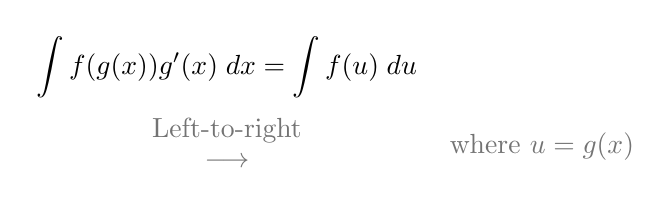
\begin{tikzpicture}
\draw (0,0) node {$\displaystyle{\int f(g(x))g'(x) \; dx = \int f(u) \; du}$};
\draw [gray!110] (0,-0.8) node {Left-to-right};
\draw [gray!110] (0,-1.2) node {$\longrightarrow$};
\draw [gray!110] (4,-1) node {where $u = g(x)$};
\end{tikzpicture}
\end{center}
Sometimes it is useful to work ``\textbf{right-to-left}'' instead. 
\begin{center}
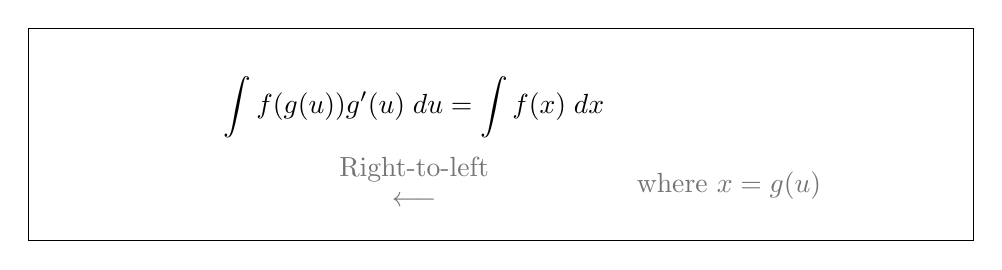
\begin{tikzpicture}
\def\x{-1.1};
\draw (0+\x,0) node {$\displaystyle{\int f(g(u))g'(u) \; du = \int f(x) \; dx}$};
\draw [gray!110] (0+\x,-0.8) node {Right-to-left};
\draw [gray!110] (0+\x,-1.2) node {$\longleftarrow$};
\draw [gray!110] (4+\x,-1) node {where $x = g(u)$};
\draw (-6,-1.7) -- (6,-1.7) -- (6,1) -- (-6,1) -- cycle;
\end{tikzpicture}
\end{center}
In right-to-left substitution, we first match our function to the expression on the right hand side. This time, instead of having $u = g(x)$, we have $x = g(u)$; i.e., $x$ is a function of $u$ now, so we can write $x(u)$ and $x'(u)$ (treating $x$ as a function) the same way we would have written $u(x)$ and $u'(x)$ when we did left-to-right substitution (when $u$ was a function of $x$). So, another way to write the right-to-left substitution rule is
\[
\int f(x(u))x'(u) \; du = \int f(x) \; dx
\]
Or another alternative notation is
\[
\int f(x(u))\frac{dx}{du} \; du = \int f(x) \; dx
\]
Again, the way we write it isn't important as long as we understand what the rule is saying. Also keep in mind that, really, left-to-right and right-to-left substitution are the same rule, we just write them differently because we use them differently (we like to have the $u$ on the side that we are moving towards).

\subsubsection{Example: proof of antiderivative of $\boldsymbol{\frac{1}{x}}$}

\noindent In section \ref{log no proof}, we stated that $\frac{d}{dx}\brac{\ln(x)} = \frac{1}{x}$, then we used this claim in section \ref{derivativetable1} to show that $\int \frac{1}{x} \; dx = \ln(x)$. We still have not proven the original claim. \\

\noindent We now present a proof that $\int \frac{1}{x} \; dx = \ln(x)$, as an easy example of right-to-left substitution; the fact that $\frac{d}{dx}\brac{\ln(x)} = \frac{1}{x}$ then follows naturally, since integration (i.e., antidifferentiation) is inverse to differentiation. \\ 

\noindent This proof only uses the derivative of $\e^x$ and the fact that $\ln(x)$ is inverse to $\e^x$. \\

\noindent Let $f(x) = \frac{1}{x}$ and let $x = g(u) = \e^u$. Then
\[
g'(u) = \frac{d}{du}\brac{\e^u} = \e^u \qquad \text{and} \qquad f(g(u)) = \frac{1}{\e^u}. 
\]
Also, since $x = \e^u$, it follows that $u = \ln(x)$ (taking natural log of both sides, since natural log is inverse to exponential). Now,
\begin{align*}
\int \frac{1}{x} \; dx & = \int f(x) \; dx \tag{as $f(x) = \frac{1}{x}$} \\
	& = \int f(g(u))g'(u) \; du \tag{integration by substitution (right-to-left)} \\
	& = \int \frac{1}{\e^u} \e^u \; du \tag{plugging in our results: $f(g(u)) = \frac{1}{\e^u}$ and $g'(u) = \e^u$} \\
	& = \int 1 \; du \\
	& = u \tag{since we are integrating with respect to $u$}\\
	& = \ln(x). \tag{since $u = \ln(x)$}
\end{align*}

\section{Right-to-left substitution with definite integrals}
In section \ref{subst definite} we learned about left-to-right substitution with definite integrals. We had $u = g(x)$, and the terminals on the left hand side were $a$ and $b$. However, in right-to-left substitution we have $x = g(u)$, and we choose to label the terminals on the right $a$ and $b$. To understand it right-to-left we can write the substitution rule as:
\begin{center}
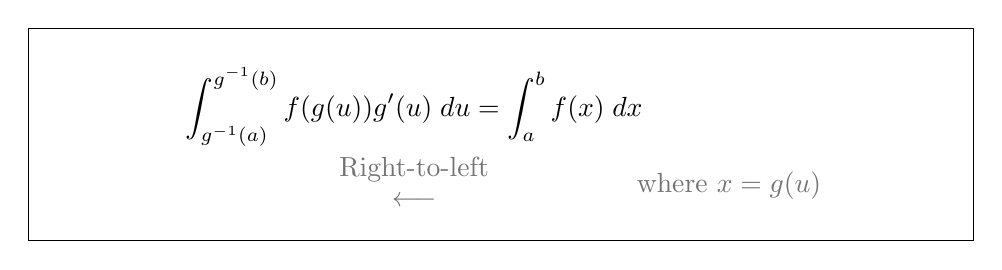
\begin{tikzpicture}
\def\x{-1.1};
\draw (0+\x,0) node {$\displaystyle{\int_{g^{-1}(a)}^{g^{-1}(b)} f(g(u))g'(u) \; du = \int_a^b f(x) \; dx}$};
\draw [gray!110] (0+\x,-0.8) node {Right-to-left};
\draw [gray!110] (0+\x,-1.2) node {$\longleftarrow$};
\draw [gray!110] (4+\x,-1) node {where $x = g(u)$};
\draw (-6,-1.7) -- (6,-1.7) -- (6,1) -- (-6,1) -- cycle;
\end{tikzpicture}
\end{center}
Once we move to the left, we need the terminals to be ``in terms of'' $u$. Since we defined $x = g(u)$, it follows that $u = g^{-1}(x)$, which is why we are using the inverse of $g$ to obtain terminals in terms of $u$. So, for example, if $x = g(u) = u + 2$, then $u = g^{-1}(x) = x - 2$ (solving for $x$). \\

\noindent In the following two sections we will use right-to-left substitution on definite integrals.
\section{Checking that the pdf of Gamma($\boldsymbol{\alpha,
\lambda}$) satisfies axiom 1} \label{gamma axiom 1}
In section \ref{pdf} we stated two conditions that need to be checked for pdfs, which are equivalent to checking probability measure axioms 1 and 2. It is easy to check that the outputs of the pdf are all positive, so we wont check that here; we just check axiom 1. We will do this using right-to-left substitution. The pdf of the gamma distribution is
\[
f(x) = \left\{ \begin{array}{ll}
\frac{\lambda^\alpha}{\Gamma(\alpha)}x^{\alpha - 1}\e^{-\lambda x} \; dx, & \; \text{if} \; x \geq 0 \smallskip \\
0, & \; \text{if} \; x < 0
\end{array}
\right.
\]
Hence we have
\[
\int_{-\infty}^\infty f(t) \; dt = \int_{0}^\infty \frac{\lambda^\alpha}{\Gamma(\alpha)}t^{\alpha - 1}\e^{-\lambda t} \; dt \tag{since $f(x) = 0$ for $x < 0$}.
\]
Let $f(x)$ be the pdf of the gamma distribution, and let $t = g(u) = \frac{u}{\lambda}$. Then $g'(u) = \frac{1}{\lambda}$ (since $\frac{1}{\lambda}$ is just a constant). Also, we can solve for $u$ in $t = \frac{u}{\lambda}$ to get $g^{-1}(t) = u = \lambda t$. \\

\noindent Now, when we do the substitution, we have to think about the terminals: Since $u = g^{-1}(t) = \lambda t$, we can see that $u \rightarrow \infty$ as $t \rightarrow \infty$ and $u = 0$ when $t = 0$, so in this case the terminals do not change when we do the substitution: 
\begin{align*}
\int_{-\infty}^\infty f(t) \; dt & = \int_0^\infty f(g(u))g'(u) \; du \tag{substitution right-to-left} \\
	& = \int_0^\infty \frac{\lambda^\alpha}{\Gamma(\alpha)}\brac{\frac{u}{\lambda}}^{\alpha - 1} \e^{-u} \frac{1}{\lambda} \; du \tag{since $g'(u) = \frac{1}{\lambda}$ and $g(u) = \frac{u}{\lambda}$} \\
	& = \int_0^\infty \frac{\lambda^\alpha}{\Gamma(\alpha)}\frac{1}{\lambda}\frac{u^{\alpha - 1}}{\lambda^{\alpha - 1}} \e^{-u} \; du  \tag{index laws, and rearranging} \\
	& = \int_0^\infty \frac{\lambda^\alpha}{\Gamma(\alpha)}\frac{1}{\lambda^\alpha} u^{\alpha - 1} \e^{-u} \; du  \tag{index laws, i.e., $\frac{1}{\lambda}\frac{1}{\lambda^{\alpha - 1}} = \frac{1}{\lambda^\alpha}$} \\
	& = \frac{1}{\Gamma(\alpha)} \int_0^\infty u^{\alpha - 1} \e^{-u} \; du  \tag{cancelling the two $\lambda^\alpha$ and using linearity} \\
	& = \frac{1}{\Gamma(\alpha)}\Gamma(\alpha) \tag{definition of the gamma function} \\
	& = 1.
\end{align*}
So $\int_{-\infty}^\infty f(t) \; dt = 1,$ as required. \\

\noindent Notice that the choice of substitution, $t = \frac{u}{\lambda}$, generated a factor of $1/\lambda^\alpha$, which resulted in the powers of $\lambda$ cancelling eachother out. In general, for the above integral, a substitution of $t = cu$, for any positive real number choice of $c$, will produce a factor of $c^\alpha$. The powers of $\lambda$ don't cancel unless $c = \frac{1}{\lambda}$, but we can still use index laws to bring $\lambda$ and $c$ together as $c^\alpha \lambda^\alpha = \brac{c \lambda}^\alpha$. \\

\noindent We will see this in action in the next section when look at why $\lambda$ is called the ``inverse scale parameter.''
%, and $\e^{-\lambda t}$ become $\e^{-\frac{\lambda}{c}u}$. This is the reason that we name $\lambda$ the ``inverse scale parameter''; we discuss this further in the next section. 

\section{Random variables and scale} \label{rate/scale gamma} \label{scale - actual description}
Suppose we have one random variable, $X$, and we wish to define another random variable, $Y$, using $X$. Recall that random variables are fuctions whose domain is the outcome space, and whose range is some subset of the real numbers. The possible outputs of $Y$ are represented by  $y$, and the possible outputs of $X$ are represented by $x$. In section \ref{def Y = g(X)} we will look at defining one variable in terms of another variable, more generally. For now, we will just look at the case, $Y = \frac{X}{c}$. Let $c$ be a positive real number. If we write $Y = \frac{X}{c}$, we mean that we take each individual output, $x$, of $X$, and from each of these obtain each output, $y$, of $Y$, by letting $y = \frac{x}{c}$.
\begin{center}
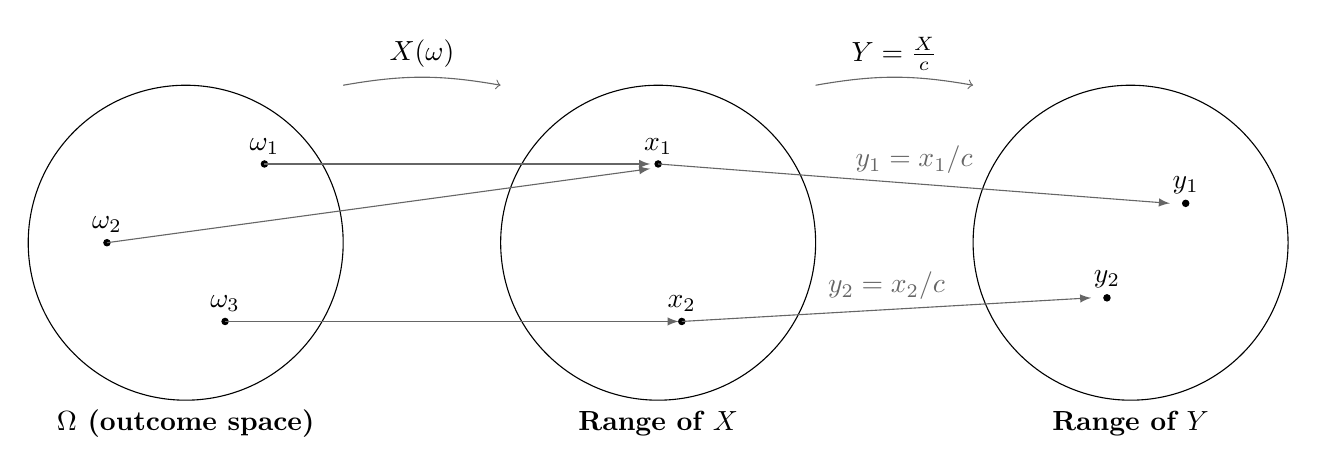
\begin{tikzpicture}
%outcome space
\draw (-6,0) circle (2cm);
\draw (-6,-2.3) node {$\boldsymbol{\Omega}$\textbf{ (outcome space)}};
\draw [fill = black] (-5,1) circle (0.04cm) node [above] {$\omega_1$};
\draw [fill = black] (-7,0) circle (0.04cm) node [above] {$\omega_2$};
\draw [fill = black] (-5.5,-1) circle (0.04cm) node [above] {$\omega_3$};

%range of X
\draw (0,0) circle (2cm);
\draw (0,-2.3) node {\textbf{Range of $\boldsymbol{X}$}};
\draw [fill = black] (0,1) circle (0.04cm) node [above] {$x_1$};
\draw [fill = black] (0.3,-1) circle (0.04cm) node [above] {$x_2$};

%range of Y
\draw (6,0) circle (2cm);
\draw (6,-2.3) node {\textbf{Range of $\boldsymbol{Y}$}};
\draw [fill = black] (6.7,0.5) circle (0.04cm) node [above] {$y_1$};
\draw [fill = black] (5.7,-0.7) circle (0.04cm) node [above] {$y_2$};

%ARROWS
%from Omega to X
\draw [gray!120, -latex] (-5,1) -- (-0.1,1);
\draw [gray!120, -latex] (-7,0) -- (-0.1,0.94);
\draw [gray!120, -latex] (-5.5,-1) -- (0.26,-1);
%from X to Y
\draw [gray!120, -latex] (0,1) -- (6.5,0.5) node [above, midway] {$y_1 = x_1/c$};
\draw [gray!120, -latex] (0.3,-1) -- (5.5,-0.7) node [above, midway] {$y_2 = x_2/c$};

%curvy arrows
\draw [gray!120, ->] (-4,2) [out=10, in =170] to (-2,2);
\draw (-3,2.4) node {$X(\omega)$};

\draw [gray!120, ->] (2,2) [out=10, in =170] to (4,2);
\draw (3,2.4) node {$Y = \frac{X}{c}$};

\end{tikzpicture}
\end{center}




\noindent So, for example, if $X = 1$, then $Y = \frac{1}{c}$, or if $X = 2.4$, then $Y = \frac{2.4}{c}$. In this way, $\set{X = a}$, for some $a$, will refer to one subset of the outcome space (i.e., one event), and consequently $\set{Y = \frac{a}{c}}$, will refer to \textit{the same} event. So, in the above graph we have $\set{Y = y_2} = \set{\omega_3}$ and $\set{Y = y_1} = \set{\omega_1,\omega_2}$. If you are having trouble thinking of random variables as functions whose domain is the outcome space, then review section \ref{sec8.10}. \\

\noindent For example, suppose that $X$ measures, in centimeters, the level of water in a reservoir after a period of rainfall. Then the event $X = 200$ corresponds to a depth of 200cm. Now, define $Y = \frac{X}{100}$. Then, when $X = 200$ we have $Y = \frac{200}{100} = 2$ units. The units of $Y$ are not centimeters, since $X = 200$ and $Y = 2$ both refer to the \textit{same event} (i.e., the same depth). There are 100 centimeters in a meter, so the units of $Y$ are meters; the water is 200cm, i.e., 2 meters, deep. The depth of the water is the same in both cases, we are just looking at it on a different \textbf{scale}; that is, $Y$ is just a \textbf{rescaled} version of $X$. \\

\noindent Now, suppose we have $X \sim$ Gamma($\alpha,\lambda$), and we define $Y = \frac{X}{c}$. Then what is the distribution of $Y$? We claim that $Y \sim$ Gamma($\alpha,c\lambda$). That is, we claim that rescaling $X$, to create $Y$, only affects the ``inverse scale parameter,'' $\lambda$; this would justify the use of the word, ``scale,'' in the naming of $\lambda$. In lecture 21 we will learn about the ``method of distributions,'' which will allow us to prove this fact, in section \ref{ex21.1}. \\

\noindent Indeed, if $X \sim$ Gamma($\alpha,\lambda$), and $Y = \frac{X}{c}$. Then $y = \frac{x}{c}$ so let $x = g(y) = cy$ (solving for $x$). So, we have $g'(y) = \frac{dx}{dy} = \frac{d}{dy}\brac{cy} = c$. Hence, we can use right-to-left substitution, almost the same as we did in section \ref{gamma axiom 1}:
\begin{align*}
P(a < X < b) & = \int_a^b \frac{\lambda^\alpha}{\Gamma(\alpha)}x^{\alpha - 1} \e^{-\lambda x} \; dx \tag{By the pdf for $X$} \\
	& = \int_{g^{-1}(a)}^{g^{-1}(b)} \frac{\lambda^\alpha}{\Gamma(\alpha)}(cy)^{\alpha - 1} \e^{-\lambda (cy)} \; \frac{dx}{dy} \; dy \tag{substitution with $x = g(y) = cy$}
\end{align*}
We had $x = g(y) = cy$, so $y = g^{-1}(x) = \frac{x}{c}$. Thus the terminals are $g^{-1}(a) = \frac{a}{c}$ and $g^{-1}(b) = \frac{b}{c}.$ Plugging these in gives
\begin{align*}
P(a < X < b) & = \int_{a/c}^{b/c} \frac{\lambda^\alpha}{\Gamma(\alpha)}(cy)^{\alpha - 1} \e^{-\lambda (cy)} \; c \; dy \tag{as $\frac{dx}{dy} = c$} \\
	& = \int_{a/c}^{b/c} \frac{\lambda^\alpha}{\Gamma(\alpha)} c^\alpha y^{\alpha - 1} \e^{-(c \lambda) y} \; dy \tag{bringing together all the factors of $c$} \\
	& =  \int_{a/c}^{b/c} \frac{(c \lambda)^\alpha}{\Gamma(\alpha)} y^{\alpha - 1} \e^{-(c \lambda)y} \; dy \;\;\;\;\;\;\;\;\;\;\;\; (\bigstar) \tag{since $c^\alpha \lambda^\alpha = (c \lambda)^\alpha$}
\end{align*}
But now notice that if we let $Y \sim$ Gamma($\alpha,c \lambda)$ then
\begin{align*}
P(a/c < Y < b/c) & =  \int_{a/c}^{b/c} \frac{(c \lambda)^\alpha}{\Gamma(\alpha)} y^{\alpha - 1} \e^{-(c \lambda)y} \; dy \tag{By the pdf of Gamma($\alpha,c \lambda$)} \\
	& = P(a < X < b). \tag{by $\bigstar$}
\end{align*}
This means that if $Y = \frac{X}{c}$, then the probability of $X$ falling in a particular interval, $[a,b]$, is equal to the probability of $Y$ falling in the interval $[a/c,b/c]$, as long as we assume that $Y \sim$ Gamma($\alpha,c \lambda)$. \\

\noindent This has not been a proof that $Y \sim$ Gamma($\alpha,c \lambda)$, we will do that proof in lecture 21 after we learn the ``method of distributions''. However, it does tell us something that we would intuitively expect from scaling a variable: If a reservoir of water is between 200cm and 300cm deep with probability $p$, then the same reservoir is between 2m and 3m deep with the same probability, $p$. The graphs of the distributions are different only because we decided to use a variable that was scaled differently (which resulted in a different value of the inverse scale parameter). It also helps us understand the use of the word ``inverse'' in this context; multiplying $\lambda$ by $c$ corresponded to dividing $X$ by $c$: Two numbers are the \textbf{\textit{multiplicative} inverses} of eachother when multiplying them together gives 1 (and indeed $c\times\frac{1}{c} = 1$).  \label{multiplicative inverses}


